% =====================================================================
%  Chapter 28 — The Roadmap, and Why the Answer Matters
% =====================================================================

\chapter{The Roadmap to 2040}
\label{ch:roadmap}

The last chapter gives the schedule and the closing argument. The schedule
is a decade long and it is written in the present tense, because the
decisions that determine it are being made now.

\begin{figure}[!htbp]
\centering
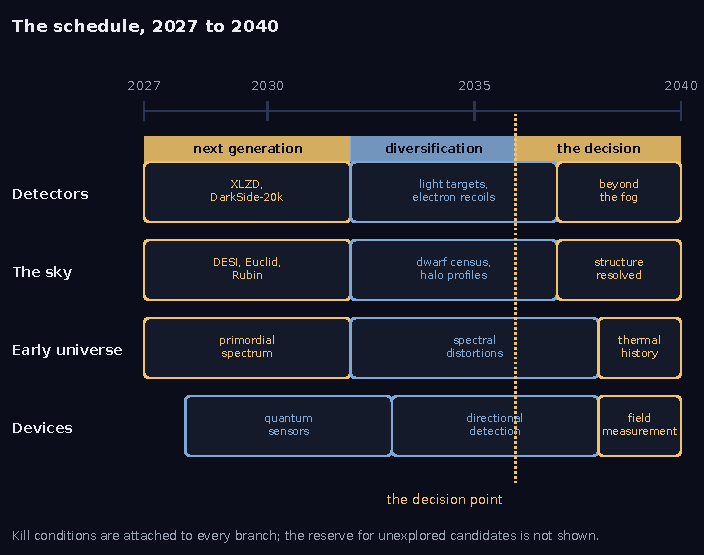
\includegraphics[width=\textwidth]{../figures/fig_roadmap.pdf}
\caption{The schedule, 2027 to 2040, by programme. The rows are the four
areas of the portfolio of Chapter~\ref{ch:portfolio}; the phase bars are
the three periods of the argument in this section. The reserve for
exploratory work discussed at the end of the chapter is not shown.}
\label{fig:roadmap}
\end{figure}

\section{2027 to 2030: the generation that is already funded}Three things
happen in this period, and none of them requires a new decision.

The \emph{next-generation suite} comes online. XLZD, the combination of the
LUX-ZEPLIN and XENONnT programmes, and DarkSide-20k, are both in
construction with multi-tonne targets and both will be operating at
sensitivities a factor of a few beyond the current limits. The practical
consequence is that the 248~keV candidate of Chapter~\ref{ch:event248} will be
tested by a new generation with independent background control, and the
result will be known before the end of the decade.

The \emph{astrophysical programme} matures. DESI continues to grow, the
Euclid and Rubin surveys begin their proper operations, and the combination
of wide-field imaging with spectroscopy turns the $S_8$ and dark energy
questions into measurements rather than comparisons. The Milky Way's halo
velocity distribution and the local density are measured by the
astrophysical route and, if the laboratory route is funded, by the direct
route as well.

The \emph{early universe programme} should be running at full strength, and
in 2026 it is not. The measurement of the primordial power spectrum at small
scales, the CMB spectral distortion constraint on the primordial black hole
mass function, and the thermal history constraints require no new facility.
They require a community, and they have one tenth the resources of the
direct-detection community.

\begin{takeaway}{The schedule decision that has to be made now}
The next-generation detectors are funded, built, and will deliver. The
question that is open in 2026 is whether the resources for the two
diversifications that the neutrino floor demands --- light targets and
electron recoils on one side, quantum devices and directional detection on
the other --- are committed in time for them to contribute to the decision
that will be made around 2032 rather than around 2040. A programme that
starts in 2030 produces its results in 2037. This is the single most
consequential scheduling fact in the book, and it is cheap to act on now and
expensive to act on later.\end{takeaway}

\section{2030 to 2035: diversification and the device revolution}This period is
where the strategy of Chapter~\ref{ch:portfolio} either has been executed
or has not.

The \emph{light-target and electron-recoil} programme should be producing its
results, and the sub-GeV region of parameter space should be either closed
or open depending on what the detectors show. The \emph{directional}
programmes should have their first results, and the local halo velocity
distribution should be measured to a precision that propagates into every
laboratory limit as a known quantity rather than a nuisance parameter.

The \emph{quantum device} programme should be the surprise of the decade,
if it is funded. It is the only route in the book to a measurement that is
qualitatively different in kind, and it is the only route that produces a
technological capability as a by-product.

And the \emph{small-scale structure} programme should have produced the
measurements that decide between cold, warm and wave-like dark matter: the
dwarf galaxy census at the necessary depth, the halo concentration-mass
relation, the Milky Way's central profile at the necessary precision, and
the CMB lensing power spectrum at high multiplicity.

\section{2035 to 2040: the decision}By 2035 the field will be in one of four
states, and the state determines what the following decade is for.

In the first state, a particle has been detected and confirmed, and the
programme of Chapter~\ref{ch:discovery} is running: abundance fraction,
production mechanism, and the small-scale problems still standing. In the
second state, the candidate space has been closed down to a small region
that no experiment in the portfolio can reach --- the genuinely awkward
state, which is the one the field has never before been in, and which
Chapter~\ref{ch:origin} describes as the case for a model-level programme
rather than a search programme. In the third state, the cosmological
measurements have produced a result of the kind DESI hinted at, and the
priority has shifted from particle dark matter to the dark sector as a
whole. In the fourth state, nothing has been found and the constraints have
improved by an order of magnitude, and the field must decide whether to
continue, and the answer to that question is itself a decision that has to
be made in advance.

The fourth state deserves a plan now, because it is the state with no
advocates. The right response is to have decided in advance what the
decision rule is, which is the subject of Chapter~\ref{ch:criteria}: each
candidate has a kill condition, and the aggregate of the kill conditions is
the field's decision rule for the 2040s.

\section{The case for the exploratory reserve}Every table of this kind has a blind
spot, and it is the candidates that nobody has thought of yet. The 248~keV
candidate was not predicted by anybody's roadmap. The detection of the
correlations between high-redshift galaxies and the distribution of dark
matter haloes is recent. The unexpected results of the last five years have
all come from outside the plan.

The recommendation is unfashionable and simple: a reserve of exploratory
funding, allocated to measurements that are not tied to a candidate and not
tied to a facility, on the basis that the most valuable result of the last
decade --- the discovery of the small-scale problems, which redirected the
field --- was not planned by anybody.

\section{Why the answer matters}The final question of the book is the one in its
subtitle, and it deserves a serious answer rather than a rhetorical one.

The reason this question is urgent is not that dark matter is interesting.
It is that the current state of knowledge about the universe is a small
fraction of what is knowable, and that fraction is shrinking in relative
terms as the questions get harder. Dark matter is the largest single item in
that knowledge debt. A civilisation that intends to be long-lived --- to
push itself into the future and to ensure its own survival --- needs to
convert at least some of that debt into knowledge, because knowledge is the
only asset that compounds.

There are four concrete ways in which the answer matters, and the fourth is
the largest.

The first is \emph{energy}. Humanity's energy budget is a nineteenth-century
technology. Fusion is the obvious candidate for the next one, and fusion is
a materials problem before it is a physics problem: a fusion reactor that
can be built from materials we can mine is a different prospect from one
that requires exotic isotopes. The energy content of the local dark matter
is immense, as Chapter~\ref{ch:harvest} showed, and the coupling that would
let us touch it does not exist in nature. That does not settle the energy
question; it settles the question of whether dark matter will be part of the
answer, and the answer is no.

The second is \emph{structure}. Dark matter is what built the galaxies, and
the galaxies are what hold the stars. The cusp-core and too-big-to-fail
problems are therefore not curiosities about dwarf galaxies; they are
statements about how structure assembles, and the same physics governs
structure formation at every scale, including in the artificial structures
that a long-horizon civilisation will build. A field that cannot predict
where a halo's mass ends up cannot predict where a structure ends.

The third is \emph{method}. The dark matter case is the clearest worked
example in modern physics of how a knowledge claim is actually secured and
lost. Twenty years of null results, four anomalies that did not replicate,
one live candidate, a discovery standard written down and applied, and a
look-elsewhere correction that turned a 3.4 sigma local excess into a 2.6
sigma global one. The method that produced the knowledge is: state the
standard in advance, apply it to your own results, publish the raw data, and
treat replication as the price of belief. That method is worth more than the
answer, because it is the only thing that has been reliable.

The fourth is \emph{scale}. The dark matter question is not a niche. It is
the largest object in the universe, and the field's inability to say what it
is is a measure of how little we know about the physical world we live in.
The stakes are not rhetorical. A long-horizon civilisation inherits two
kinds of problems: the ones it can see and the ones it cannot. Dark matter
is a fifty-one per cent of the universe that is, in the most literal sense,
invisible --- and it is the clearest example of the category of knowledge
debt that compounds. Knowing what it is would not make humanity safe. Not
knowing what it is leaves a hole in the map of a universe that humanity
intends to keep living in.

\begin{takeaway}{The book's single claim}
Dark matter is real, its abundance is known to two per cent, its identity is
not known, and the gap between those two facts is the largest single item in
humanity's knowledge debt about the universe. The field has a strategy for
closing it --- a portfolio of differentiated experiments, each with a
confirmation criterion and a kill condition --- and the strategy's first
requirement is not a detector but a decision about how the existing sky and
the existing universe are used.\end{takeaway}
